\documentclass{hw}
\usepackage{amsmath}
\usepackage{cancel}
\usepackage{nuc}
\usepackage{graphicx}

\graphicspath{ {./}}

\newcommand{\mean}{\bar}

\author{J.R. Powers-Luhn}
\date{2018/09/04}
\title{Homework \#1}

\begin{document}
%\maketitle

\problem{2.6}
    In equation 2.13, we summed up the squares of the differences between the actual value and the estimated value. This error function is the one most frequently used, but it is one of several possible error functions. Because it sums up the squares of the differences, it is not robust to outliers. What would be a better error function to implement \textit{robust regression}?

\solution
    Mean Absolute Error would minimize errors while not being dominated by outliers.

\problem{2.7}
    Derive equation 2.17: 
    \begin{align*}
        w_0 &= \mean{r} - w_1 \mean{x} \\
        w_1 &= \frac{\sum_t x^t r^t - \mean{x r} N}{\sum_t \left( x^t \right)^2 - N \mean{x}^2}
    \end{align*}

\solution
    We seek to minimize the error function:
    \begin{align*}
        E(w_1, w_0 | X) = \frac{1}{N} \sum_{t=1}^N \left[ r^t - \left( w_1 x^t + w_0 \right) \right]
    \end{align*}

    To do this, we set the derivative $\frac{d}{dw_i} E(X)$ equal to zero. First, $w_0$:

    \begin{align*}
        0 &= \frac{d}{d w_0} \frac{1}{N} \sum_t^N \left[ r^t - \left( w_1 x^t + w_0 \right) \right]^2 \\
        &= \frac{2}{N} \sum_t^N \left( r^t - w_1 x^t - w_0 \right) \\
        &= 2 \frac{1}{N} \left[ \sum_t r^t - \sum_t w_1 x^t - \sum_t w_0 \right] \\
        \bar{r} - w_1 \bar{x} &= \frac{w_0 N}{N} \\
        w_0 &= \bar{r} - w_1 \bar{x}
    \end{align*}

    Then $w_1$:

    \begin{align*}
        0 &= \frac{d}{d w_1} \left( \frac{1}{N} \sum_t^N \left[ r^t - \left( w_1 x^t + w_0 \right) \right]^2 \right) \\
        &= \frac{1}{N} \frac{d}{dw_1} \sum^N_t \left[ (r^t)^2 - 2 r^t (w_1 x^t + w_0) + (w_1x^t + w_0)^2  \right] \\
        &= \sum_t^N \left[ -2 r^t w_1 x^t + w_1^2 (x^t)^2 2(w_1 x^t w_0) \right] \\
        \sum_t^N 2 w_1 (x^t)^2 &= \sum_t^N \left[ 2 r^t x^t - 2 x^t w_0 \right] \\
        &= \sum_t^N \left[ 2 r^t x^t - 2 x^t (\bar{r} - w_1 \bar{x}) \right] \\
        w_1 &= \frac{\sum_t x^t r^t - \mean{x r} N}{\sum_t \left( x^t \right)^2 - N \mean{x}^2}
    \end{align*}

\problem{2.9}
    Show that the VC dimension of the triangle hypothesis class is 7 in two dimensions.  (Hint: For best separation, it is best to place the seven points equidistant on a circle.)

\solution
    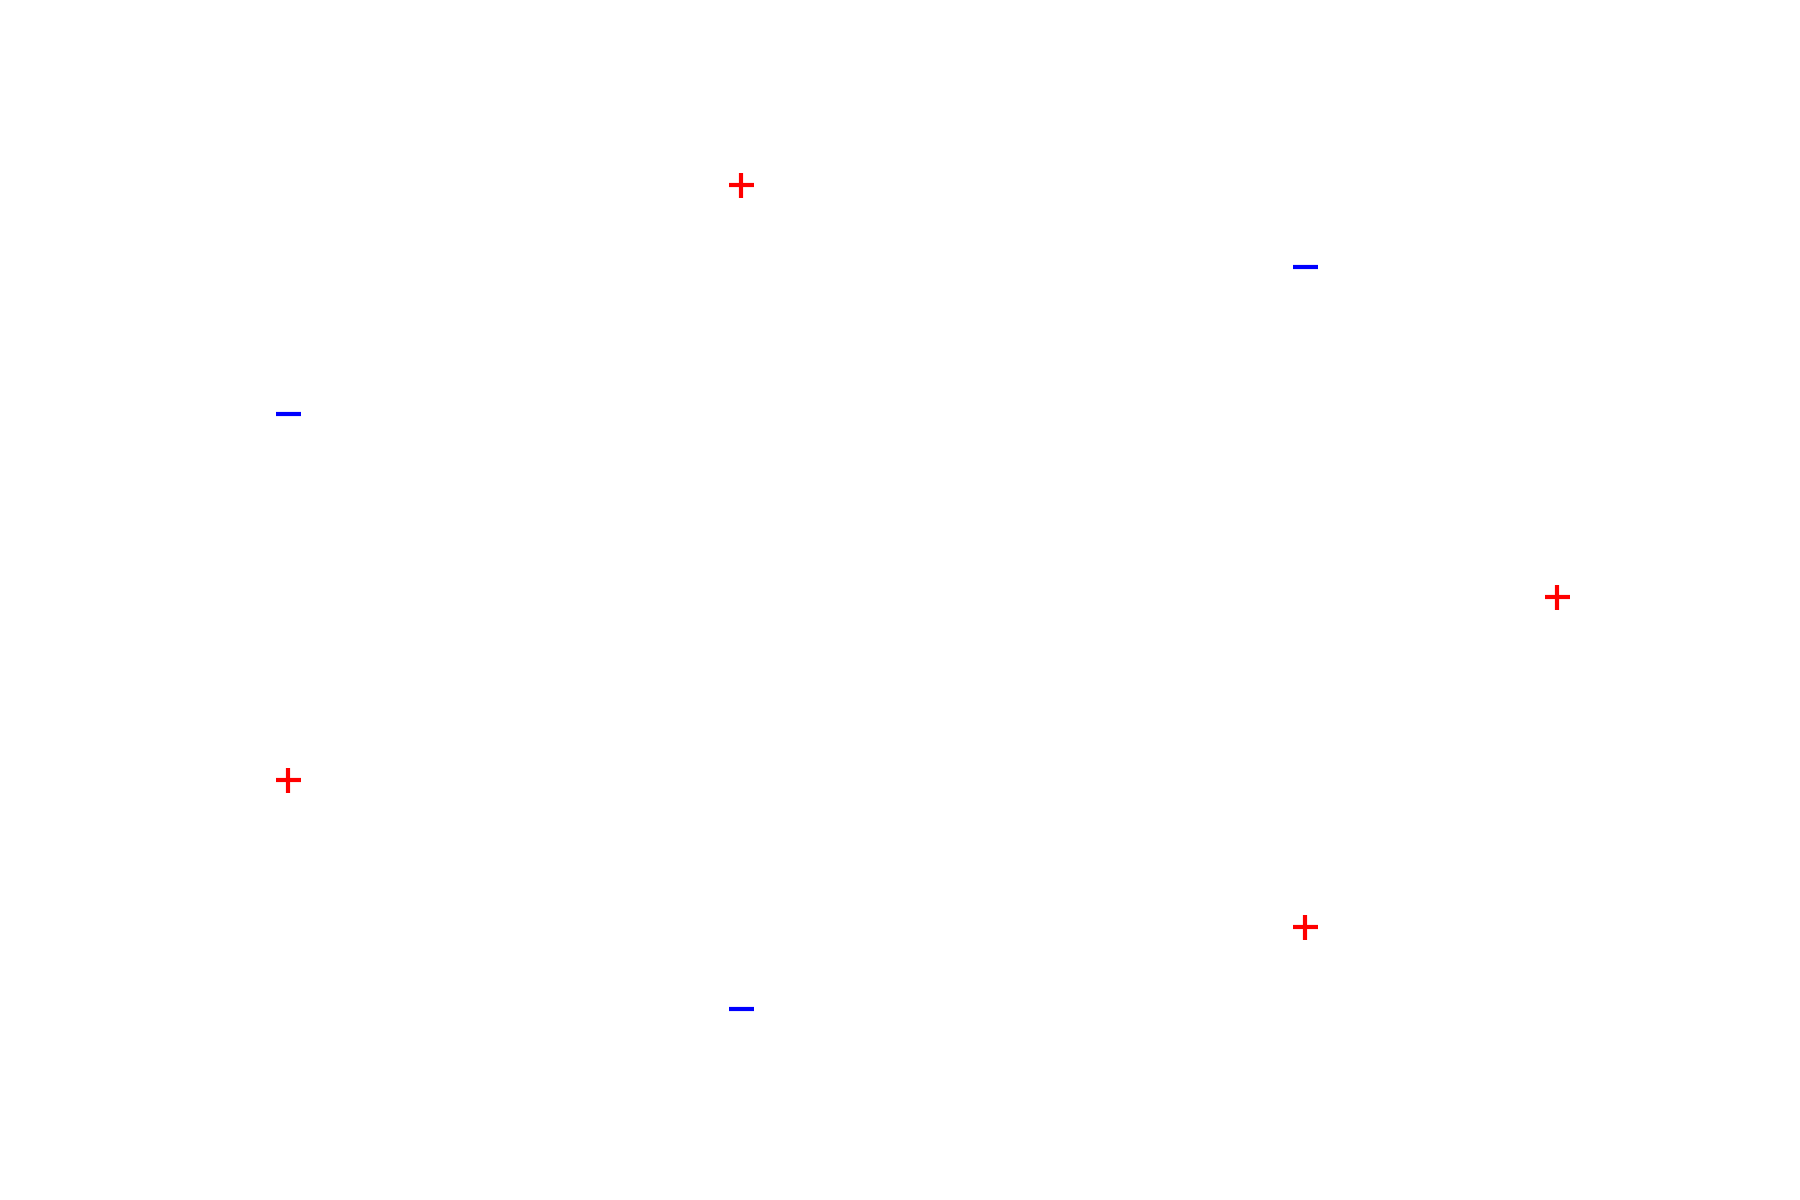
\includegraphics{better_circle_of_stars7}

    In the case of 7 points it is fairly obvious that there exists an arrangement that allows for any combination of points to be included or excluded from a hypothesis. We can therefore conclude that the VC class of this hypothesis is at least 7.

    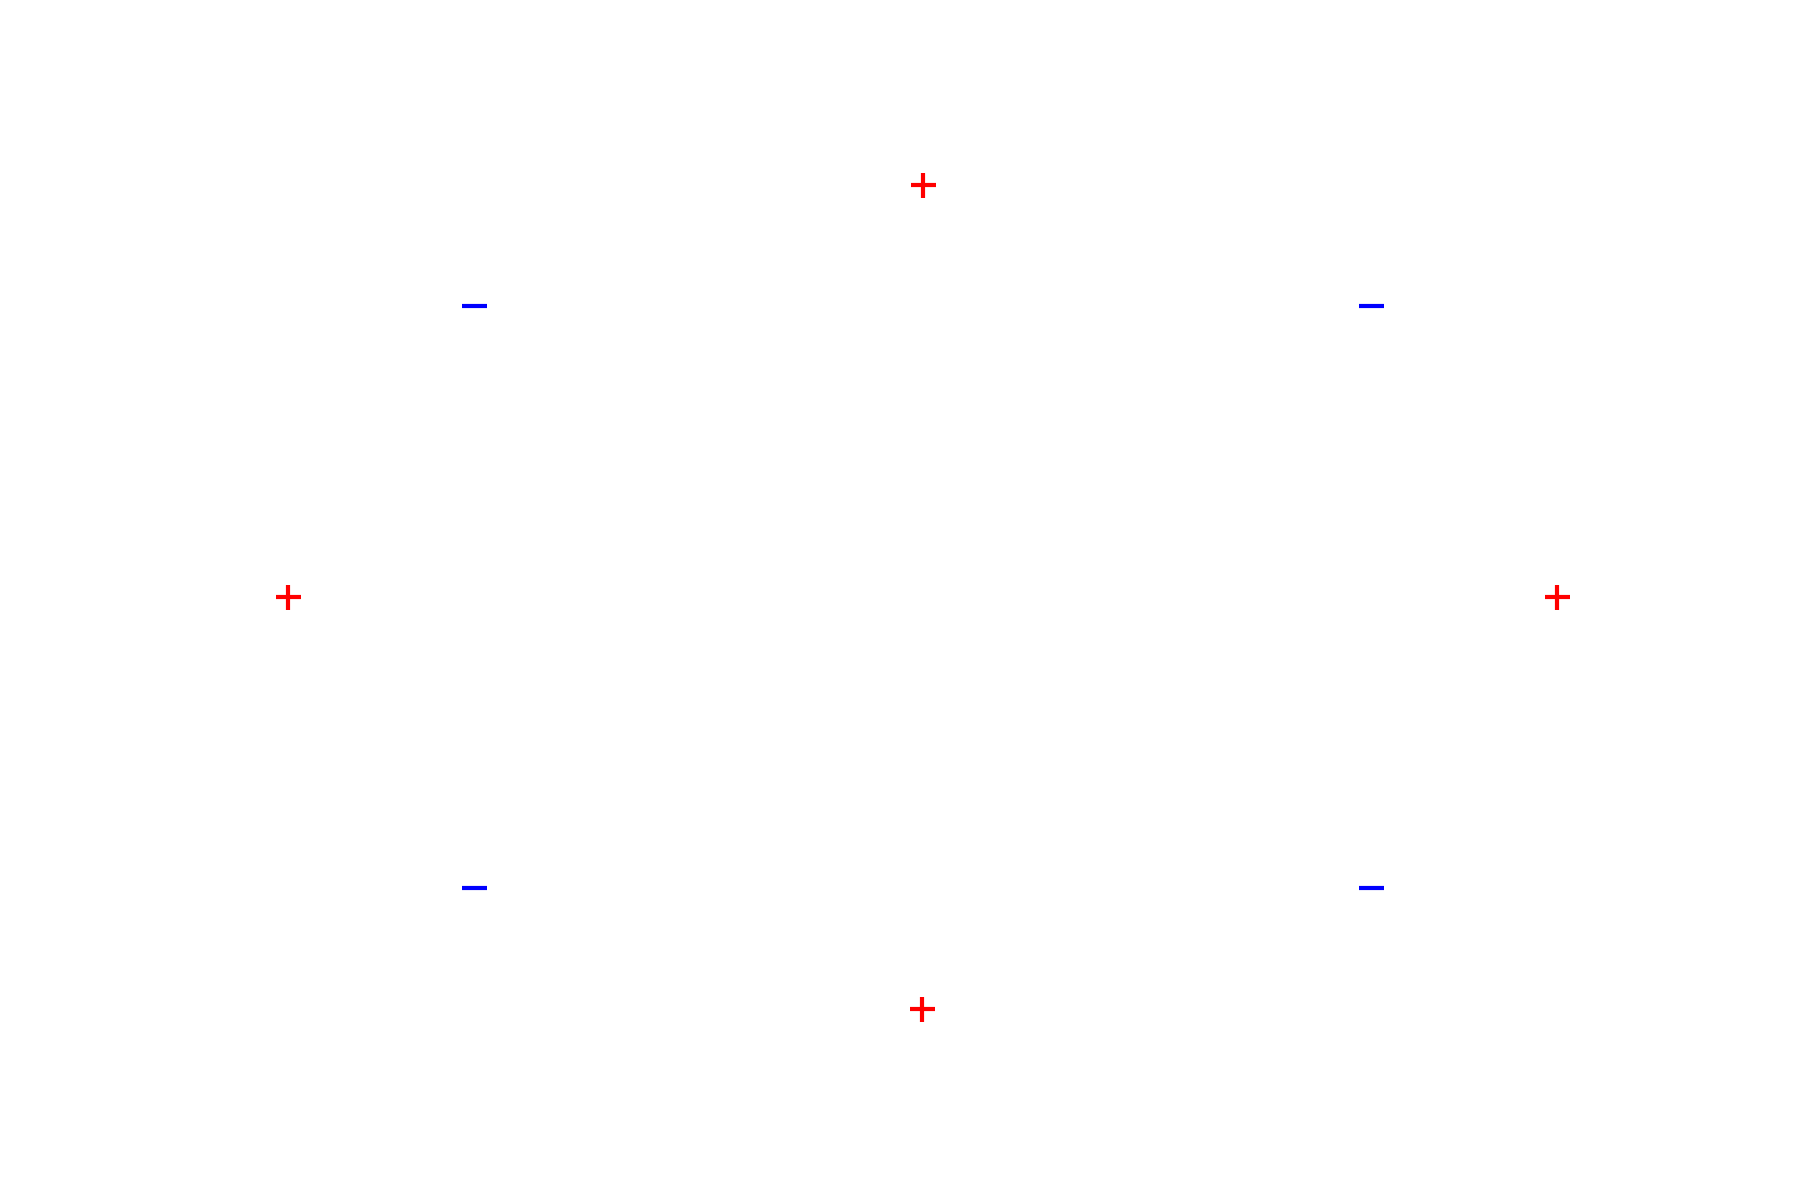
\includegraphics{better_circle_of_stars8}

    This suggests that there is no grouping that allows all positive cases to be included while excluding all negative cases. No triangle can account for all possible groupings of these points, and therefore we know that the VC class of this hypothesis is less than 8.

\problem{2.10}
    Assume as in exercise 8 that our hypothesis class is the set of lines. Write down an error function that not only minimizes the number of misclassifications but also maximizes the margin.

\solution
    We wish to devise an error function which minimizes the distance from our points to our hypothesis line:

    $$ \sum_i^N C_i \frac{\left| a x_i + b y_i +c \right|}{\sqrt{a^2 + b^2}} $$

    Where $C_i$ is the classification function, -1 for members of class 0, +1 for members of class 1.
    

\problem{2.11}
    One source of noise is error in the labels. Can you propose a method to find datapoints that are highly likely to be mislabeled?

\solution
    One method could be to train an algorithm on a number of different subsets of the data and see how often points are mislabelled. This sampling should account for random error, though it would still be vulnerable to systemic error.

\end{document}